\documentclass{standalone}
\usepackage{tikz}
\usetikzlibrary{patterns, positioning}
\usetikzlibrary{shapes.misc}
\usepackage[outline]{contour}
\contourlength{1.5pt} 


\begin{document}
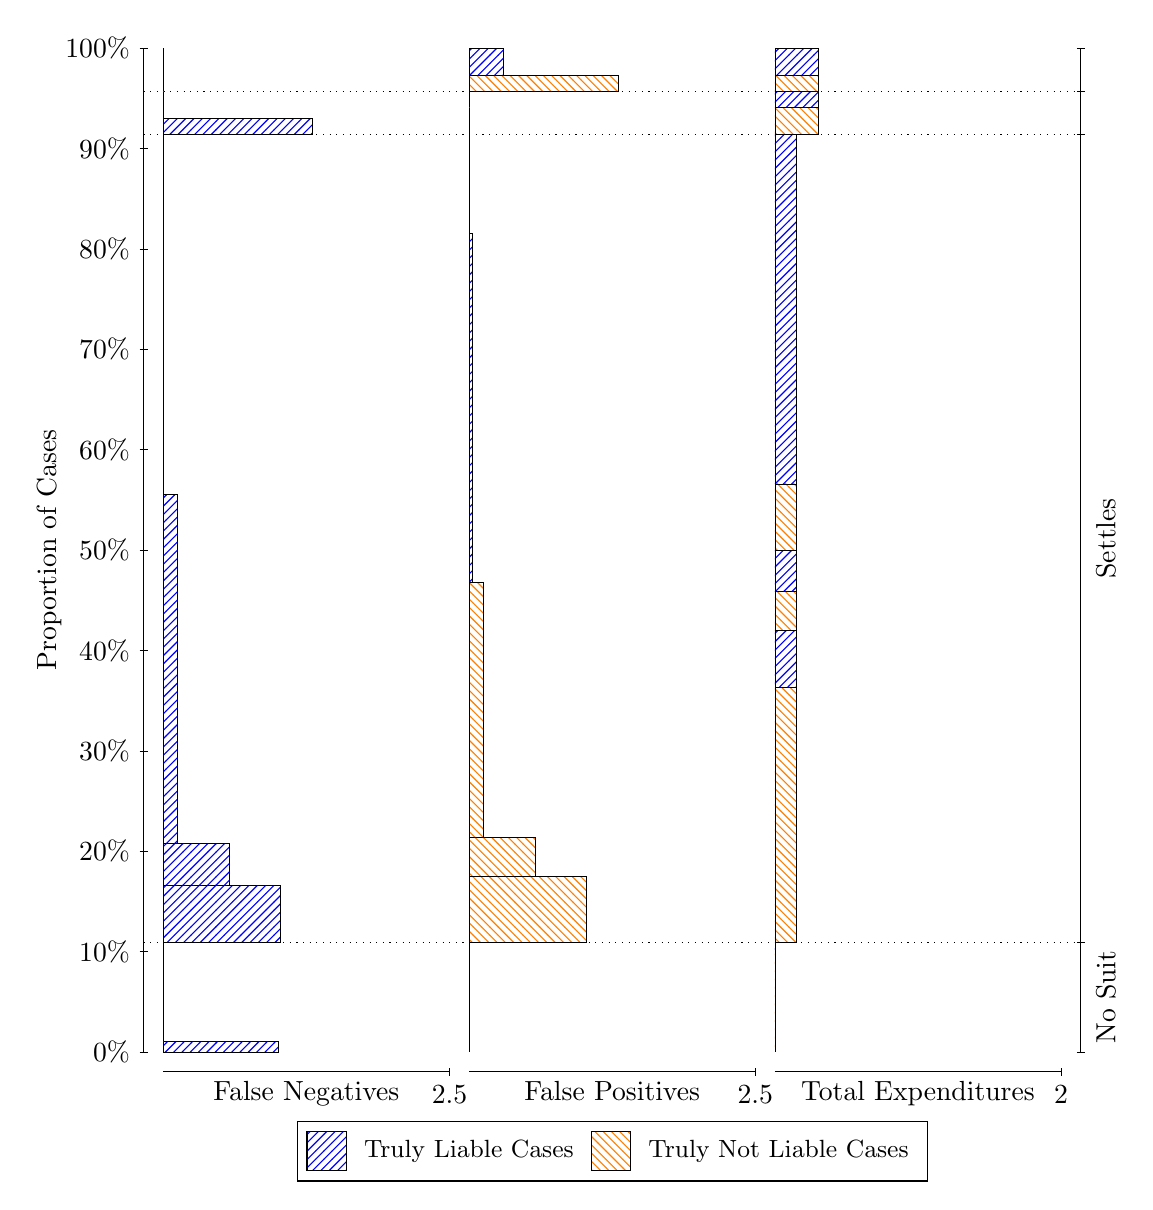
\begin{tikzpicture}
\draw[black, very thin] (1.5,1.75) -- (1.5,14.5);
\node[rotate=90, text=black, anchor=center] at (0.3, 8.125) {Proportion of Cases};
\draw[black, very thin] (1.45,1.75) -- (1.55,1.75);
\node[text=black, anchor=east] at (1.45, 1.75) {0\%};
\draw[black, very thin] (1.45,3.025) -- (1.55,3.025);
\node[text=black, anchor=east] at (1.45, 3.025) {10\%};
\draw[black, very thin] (1.45,4.3) -- (1.55,4.3);
\node[text=black, anchor=east] at (1.45, 4.3) {20\%};
\draw[black, very thin] (1.45,5.575) -- (1.55,5.575);
\node[text=black, anchor=east] at (1.45, 5.575) {30\%};
\draw[black, very thin] (1.45,6.85) -- (1.55,6.85);
\node[text=black, anchor=east] at (1.45, 6.85) {40\%};
\draw[black, very thin] (1.45,8.125) -- (1.55,8.125);
\node[text=black, anchor=east] at (1.45, 8.125) {50\%};
\draw[black, very thin] (1.45,9.4) -- (1.55,9.4);
\node[text=black, anchor=east] at (1.45, 9.4) {60\%};
\draw[black, very thin] (1.45,10.675) -- (1.55,10.675);
\node[text=black, anchor=east] at (1.45, 10.675) {70\%};
\draw[black, very thin] (1.45,11.95) -- (1.55,11.95);
\node[text=black, anchor=east] at (1.45, 11.95) {80\%};
\draw[black, very thin] (1.45,13.225) -- (1.55,13.225);
\node[text=black, anchor=east] at (1.45, 13.225) {90\%};
\draw[black, very thin] (1.45,14.5) -- (1.55,14.5);
\node[text=black, anchor=east] at (1.45, 14.5) {100\%};

\draw[black, very thin] (13.4,1.75) -- (13.4,14.5);
\draw[black, very thin] (13.35,1.75) -- (13.45,1.75);
\node[anchor=west] at (13.35, 1.75) {};
\draw[black, very thin] (13.35,3.1433) -- (13.45,3.1433);
\node[anchor=west] at (13.35, 3.1433) {};
\draw[black, very thin] (13.35,13.402) -- (13.45,13.402);
\node[anchor=west] at (13.35, 13.402) {};
\draw[black, very thin] (13.35,13.951) -- (13.45,13.951);
\node[anchor=west] at (13.35, 13.951) {};
\draw[black, very thin] (13.35,14.5) -- (13.45,14.5);
\node[anchor=west] at (13.35, 14.5) {};

\draw[black, very thin, pattern color=blue, pattern=north east lines] (1.75,1.75) rectangle (3.2033,1.8849);
\draw[black, very thin, pattern color=orange, pattern=north west lines] (1.75,1.8849) rectangle (1.75,3.1433);
\draw[black, very thin, pattern color=blue, pattern=north east lines] (1.75,3.1433) rectangle (3.2397,3.8665);
\draw[black, very thin, pattern color=blue, pattern=north east lines] (1.75,3.8665) rectangle (2.5857,4.3959);
\draw[black, very thin, pattern color=blue, pattern=north east lines] (1.75,4.3959) rectangle (1.9317,8.8346);
\draw[black, very thin, pattern color=orange, pattern=north west lines] (1.75,8.8346) rectangle (1.75,13.402);
\draw[black, very thin, pattern color=blue, pattern=north east lines] (1.75,13.402) rectangle (3.6393,13.606);
\draw[black, very thin, pattern color=orange, pattern=north west lines] (1.75,13.606) rectangle (1.75,13.951);
\draw[black, very thin, pattern color=orange, pattern=north west lines] (1.75,13.951) rectangle (1.75,14.155);
\draw[black, very thin, pattern color=blue, pattern=north east lines] (1.75,14.155) rectangle (1.75,14.5);
\draw[black, very thin, pattern color=orange, pattern=north west lines] (5.6333,1.75) rectangle (5.6333,3.0084);
\draw[black, very thin, pattern color=blue, pattern=north east lines] (5.6333,3.0084) rectangle (5.6333,3.1433);
\draw[black, very thin, pattern color=orange, pattern=north west lines] (5.6333,3.1433) rectangle (7.123,3.9821);
\draw[black, very thin, pattern color=orange, pattern=north west lines] (5.6333,3.9821) rectangle (6.469,4.4762);
\draw[black, very thin, pattern color=orange, pattern=north west lines] (5.6333,4.4762) rectangle (5.815,7.7111);
\draw[black, very thin, pattern color=blue, pattern=north east lines] (5.6333,7.7111) rectangle (5.6697,12.15);
\draw[black, very thin, pattern color=blue, pattern=north east lines] (5.6333,12.15) rectangle (5.6333,13.402);
\draw[black, very thin, pattern color=orange, pattern=north west lines] (5.6333,13.402) rectangle (5.6333,13.747);
\draw[black, very thin, pattern color=blue, pattern=north east lines] (5.6333,13.747) rectangle (5.6333,13.951);
\draw[black, very thin, pattern color=orange, pattern=north west lines] (5.6333,13.951) rectangle (7.5227,14.155);
\draw[black, very thin, pattern color=blue, pattern=north east lines] (5.6333,14.155) rectangle (6.0693,14.5);
\draw[black, very thin, pattern color=orange, pattern=north west lines] (9.5167,1.75) rectangle (9.5167,3.0084);
\draw[black, very thin, pattern color=blue, pattern=north east lines] (9.5167,3.0084) rectangle (9.5167,3.1433);
\draw[black, very thin, pattern color=orange, pattern=north west lines] (9.5167,3.1433) rectangle (9.7892,6.3783);
\draw[black, very thin, pattern color=blue, pattern=north east lines] (9.5167,6.3783) rectangle (9.7892,7.1014);
\draw[black, very thin, pattern color=orange, pattern=north west lines] (9.5167,7.1014) rectangle (9.7892,7.5956);
\draw[black, very thin, pattern color=blue, pattern=north east lines] (9.5167,7.5956) rectangle (9.7892,8.125);
\draw[black, very thin, pattern color=orange, pattern=north west lines] (9.5167,8.125) rectangle (9.7892,8.9637);
\draw[black, very thin, pattern color=blue, pattern=north east lines] (9.5167,8.9637) rectangle (9.7892,13.402);
\draw[black, very thin, pattern color=orange, pattern=north west lines] (9.5167,13.402) rectangle (10.062,13.747);
\draw[black, very thin, pattern color=blue, pattern=north east lines] (9.5167,13.747) rectangle (10.062,13.951);
\draw[black, very thin, pattern color=orange, pattern=north west lines] (9.5167,13.951) rectangle (10.062,14.155);
\draw[black, very thin, pattern color=blue, pattern=north east lines] (9.5167,14.155) rectangle (10.062,14.5);
\draw[black, dotted] (1.5,3.1433) -- (13.4,3.1433);
\draw[black, dotted] (1.5,13.402) -- (13.4,13.402);
\draw[black, dotted] (1.5,13.951) -- (13.4,13.951);
\draw[black, very thin] (1.75,1.5) -- (5.3833,1.5);
\node[text=black, anchor=north] at (3.5667, 1.5) {False Negatives};
\draw[black, very thin] (5.3833,1.45) -- (5.3833,1.55);
\node[text=black, anchor=north] at (5.3833, 1.45) {2.5};

\draw[black, very thin] (5.6333,1.5) -- (9.2667,1.5);
\node[text=black, anchor=north] at (7.45, 1.5) {False Positives};
\draw[black, very thin] (9.2667,1.45) -- (9.2667,1.55);
\node[text=black, anchor=north] at (9.2667, 1.45) {2.5};

\draw[black, very thin] (9.5167,1.5) -- (13.15,1.5);
\node[text=black, anchor=north] at (11.333, 1.5) {Total Expenditures};
\draw[black, very thin] (13.15,1.45) -- (13.15,1.55);
\node[text=black, anchor=north] at (13.15, 1.45) {2};

\node[text=black, centered, rotate=90] at (13.72, 2.4467) {\contour{white}{No Suit}};
\node[text=black, centered, rotate=90] at (13.72, 8.2729) {\contour{white}{Settles}};



\draw (7.449999999999999,1.5) node[draw=none] (baseCoordinate) {};
\begin{scope}[align=center]
        \matrix[scale=0.5, draw=black, below=0.5cm of baseCoordinate, nodes={draw}, column sep=0.1cm]{
            \node[rectangle, draw, minimum width=0.5cm, minimum height=0.5cm, pattern color=blue, pattern=north east lines] {}; &
            \node[draw=none, font=\small, text=black] (B) {Truly Liable Cases}; &
            \node[rectangle, draw, minimum width=0.5cm, minimum height=0.5cm, pattern color=orange, pattern=north west lines] {}; &
            \node[draw=none, font=\small, text=black] (B) {Truly Not Liable Cases}; \\
            };
\end{scope}

\end{tikzpicture}
\end{document}